\chapter{Introduction}\label{cha:intro}

\section{Project Overview And Motivations}
Since the advent of music streaming services, they have grown steadily, resulting in an industry with approximately \$19.3 billion in revenue in 2023~\cite{IFPI}. Despite this, vinyl records have seen a resurgence in their sales~\cite{BPI}, but the need for additional hardware is a barrier for most listeners. Turntables cannot be carried around and on top of this are not cheap. This project attempts to resolve this issue by developing a virtual turntable using web technologies to allow listeners to play their vinyl collections from the convenience of their digital devices whilst attempting to emulate the feel of dropping the needle on an LP.\@

\section{Objectives}\label{sec:objectives}
The project, at its simplest, must match the capability of a physical turntable whilst being entirely on a digital device. That is it must meet the following criteria:
\begin{itemize}
    \item Play whole albums using a representation of the physical album as input
    \item Accurately determine which album is input
\end{itemize}
On top of these basic requirements, as the project is to be used on digital devices, it should meet criteria which are common to products produced in this domain:
\begin{itemize}
    \item Visually appealing user interface
    \item Intuitive and user-friendly interface
    \item Social system between users
    \item Save users collections for easier repeat listens
\end{itemize}
As an extension to the goals for the final application produced, there are certain criteria that are considered good software development practices, and these are also goals that should be met during the development.
\begin{itemize}
    \item High code quality
    \item Automated testing
    \item Automated deployment
    \item Automated dependency management
\end{itemize}

\section{Project Plan}
Effective planning is essential in software development to ensure design criteria are met and tasks are completed, even for a solo developer. In this project, an agile approach was adopted to provide greater flexibility and support iterative development with the desire for fast development, in contrast to traditional methodologies such as Waterfall \cite{5222784}. Which is a methodology better suited for projects with well-defined scope and stable requirements, and any changes to these result in additional time spent on replanning \cite{andrei2019study}.

\subsection{Planning system} \label{sec:plan-system}
A Kanban system was used to manage development tasks, offering a structured, visual approach to tracking progress. Tasks were categorised into three stages: Backlog, In Progress, and Done, as shown in Figure~\ref{fig:kanban-board}. This system provided a clear overview of remaining work while also enabling tasks to be prioritised, ensuring that more important work, such as that composing the critical functionality, was completed first.

Critically, the planning system needed to be easy to set up and use, to avoid consuming unnecessary time. For this purpose, a GitHub Project was selected, as it required minimal setup and configuration. Additionally, it integrated directly with the project repository, enabling direct links between commits, pull requests and tasks.

\begin{figure}
    \centering
    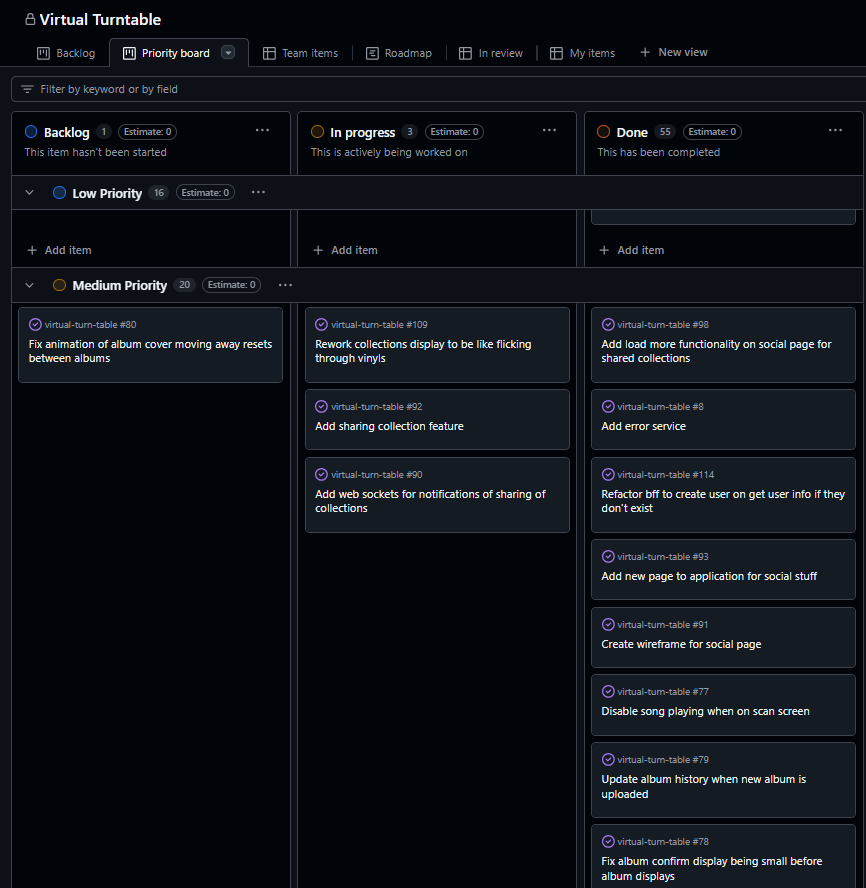
\includegraphics[width=0.65\linewidth]{figures/kanban_board.png}
    \captionsetup{justification=centering,margin=2cm}
    \caption{The Kanban board used during the project with tickets across the three columns}
    \label{fig:kanban-board}
\end{figure}

\subsection{Plan}
The plan for this project was structured into three key phases: design, development and testing, and deployment and maintenance.

\subsubsection{Design}
The first stage of the project involved finalizing the system design before commencing code development. This high-level planning approach addressed key architectural and technological decisions early in the process, ensuring a well-defined foundation. By making these decisions in advance, the need for ad hoc choices during development was minimised, reducing the risk of unintended consequences later in the project. This phase established the system's architecture, technology stack, deployment strategy, and user interface design, all of which are further detailed in Chapter~\ref{cha:design}.

\subsubsection{Development And Testing}
The development phase encompassed both the implementation of the core software and the integration of automated code quality tools to maintain consistency and reliability. A test-driven development (TDD) approach was adopted to ensure tests covered all intended functionality. This included the creation of automated tests, reducing reliance on manual testing, which was particularly useful as the project grew in size. Additionally, linters, formatters, and continuous testing were incorporated to enforce code quality standards as each commit was pushed to the repository, as further discussed in Section~\ref{sec:code-quality}.

The Kanban project planning system, outlined in Section~\ref{sec:plan-system}, played a crucial role in managing unforeseen challenges during development, such as bugs, which could be easily added to the board without disrupting the overall plan.

\subsubsection{Deployment And Maintenance}
Deployment was planned to involve hosting the system on a cloud platform to allow access from any potential user. The specific deployment method would be determined by the system’s design (Chapter~\ref{cha:design}), but a cloud-based solution was preferred due to its minimal cost for small projects and ease of configuration.

Maintenance was not a primary focus during planning; however, certain aspects were considered. Automated dependency management was planned, with bots monitoring the repository’s dependency files and updating them as new versions were released. Combined with the automated test suite, this approach ensured that dependencies could be updated with confidence and minimal manual intervention.
